\chapter{Architektur\label{chap3:Drittes-Kapitel}}

Für die Architektur der mobilen Anwendung \glqq Geogram\grqq{}, wurden die zwei Frameworks \glqq Ionic\grqq{} und \glqq Express\grqq{} und die Entwicklungs-Plattform \glqq Firebase\grqq{} verwendet.

Wie in \autoref{fig:technologie} veranschaulicht, wird das Web-Framework \glqq Ionic\grqq{} für das Frontend verwendet. Das Backend kann in zwei Bereiche unterteilt werden. Zum einen wird die Entwicklungs-Plattform \glqq Firebase\grqq{} und das Node.js Web-Framework \glqq Express\grqq{} verwendet. Genauere Informationen bezüglich der Aufteilung des Backends wird in \autoref{sec3.2:Unterpunkt-2} beschrieben.

\begin{figure}[H]
    \centering
    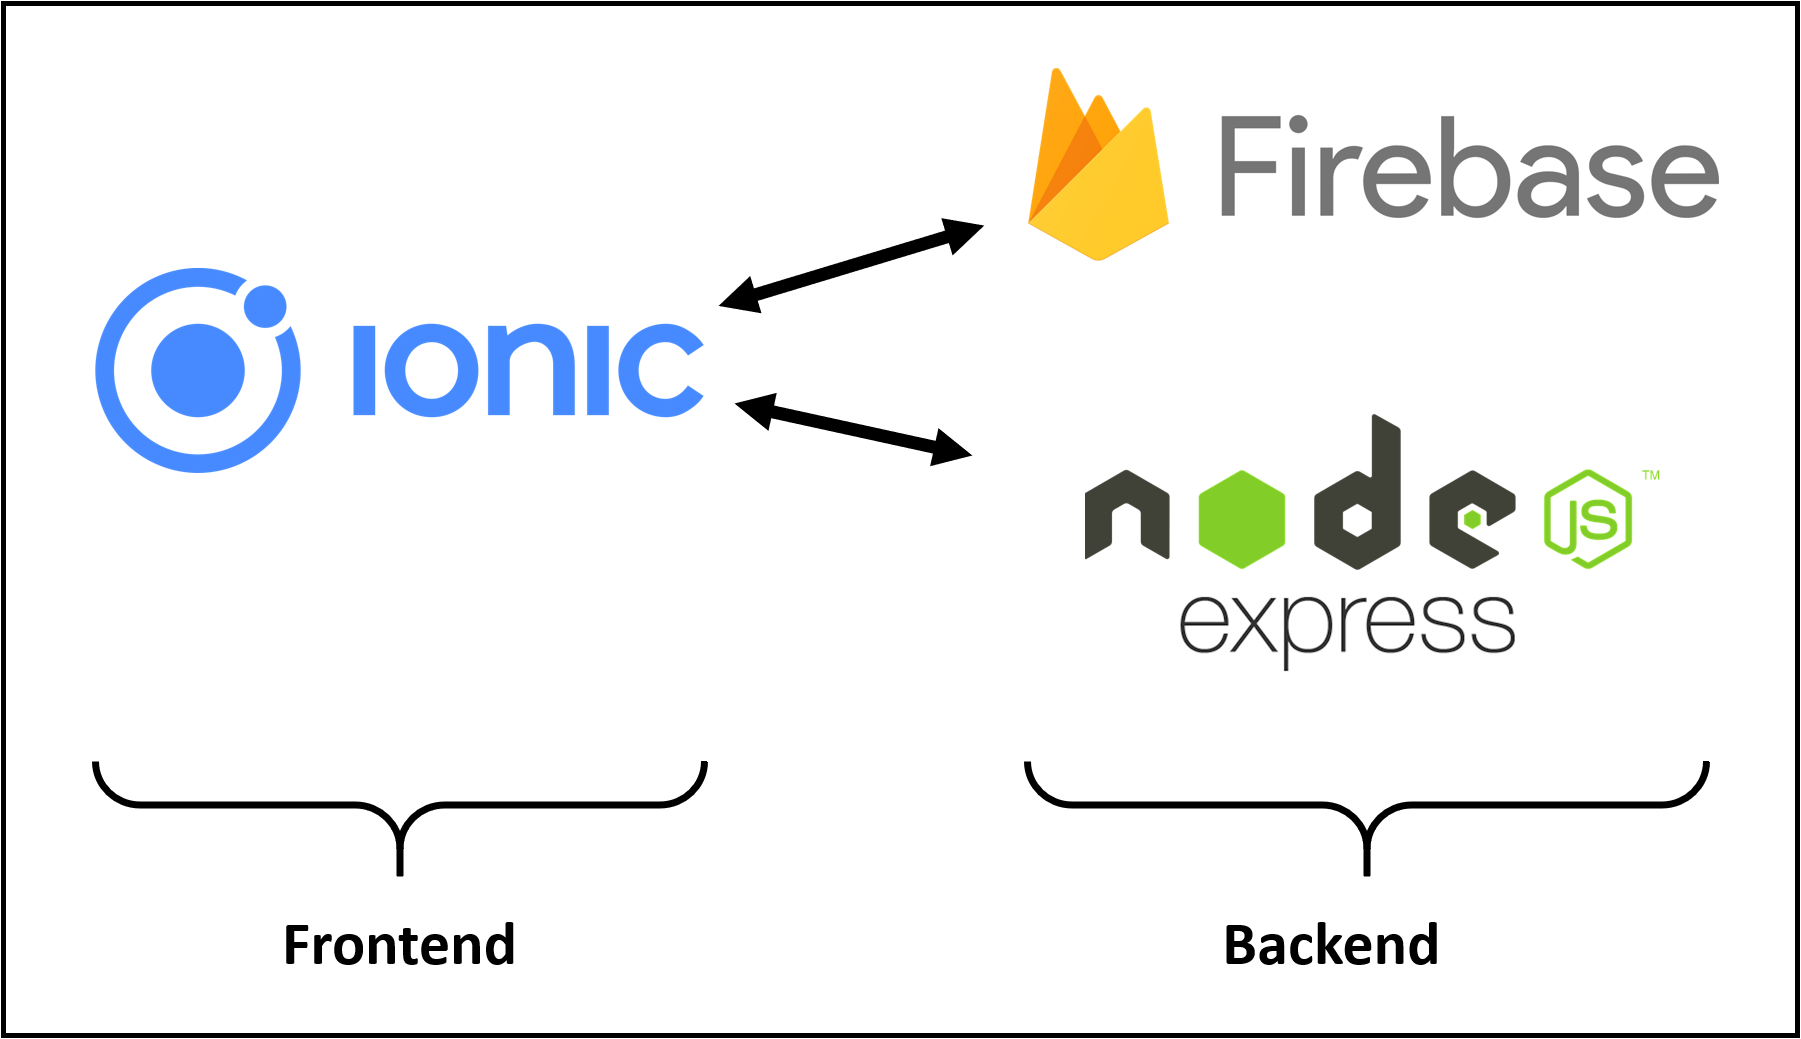
\includegraphics[width=.8\linewidth]{images/Architektur.png}
    \caption{Technologieübersicht}
    \label{fig:technologie}
\end{figure}

\section{Frontend\label{sec3.1:Unterpunkt-1}}

Inhalt

\section{Backend\label{sec3.2:Unterpunkt-2}}

Den Großteil der Backend-Aufgaben übernimmt die Entwicklungs-Platform Firebase. Verwendet wird hierfür die kostenlose \glqq Spark Plan\grqq{}-Version von Firebase. 

Die \textbf{Authentifizierung} und das \textbf{Credentialmanagent} wird hierbei vollständig von Firebase übernommen und verwaltet. Über vordefinierte Programmierschnittstellen kann man anschließend auf die Funktionen von Firebase zugreifen. Ebenso wird im kostenlosen Lizenzmodell \glqq Spark Plan\grqq{} eine Cloud-Speicherung namens \glqq \textbf{Firestore}\grqq{} angeboten. In der darin enthaltenen \textbf{Echtzeitdatenbank} stehen jedoch nur 1 GiB Speicherplatz zur Verfügung. Da sich das Kernkonzept von Geogram hauptsächlich um Fotos dreht und die finanziellen Mittel der Gruppe nicht für ein kostenpflichtiges Lizenzmodell ausreichen, wurde zusätzlich ein \textbf{Foto-Server} mithilfe des Web-Frameworks \glqq Express\grqq{} implementiert. Der Foto-Server wird von der Projekt-Gruppe selbst gehostet und beinhaltet mehr als 1 Gib Speicherplatz.

\subsection{Cloud Firestore\label{sup3.2.1:Unterpunkt-1}}

Die verwendete Firestore-Datenbank ist eine in der Cloud gehostete NoSQL-Datenbank. Über native SDKs können die iOS-, Android- und Web-Apps auf Firestore zugreifen.

\begin{wrapfigure}{r}{0.3\textwidth}
    \begin{center}
        
\includegraphics[width=0.3\textwidth]{images/firestore.png}
    \end{center}
    \caption{Speicherstruktur Firestore}
    \label{fig:storagestructure}
\end{wrapfigure}

In dem NoSQL-Datenmodell von Firestore, werden die Daten in Dokumente gespeichert, welche Felder enthalten, denen Werte zugeordnet sind. Diese Dokumente wiederrum werden in Sammlungen (collections) abgespeichert. Diese hierarchische Rangordnung der Datenspeicherung ist nochmals in \autoref{fig:storagestructure} abgebildet.

Für Geogram werden die zwei Sammlungen \glqq images\grqq{} und \glqq users\grqq{} benötigt. Wie die Bezeichnungen schon vermuten lassen, werden darin die Fotos und die Benutzer von Geogram abgespeichert.

Die Dokumente der Sammlung \glqq users\grqq{} bilden die verschiedenen Benutzerprofile von Geogram ab. Ein Benutzerprofil wird durch folgende Felder definiert:

\begin{itemize}
    \item \textbf{biography}: Eine kurze Beschreibung über den Benutzer
    \item \textbf{email}: Die E-Mail Adresse des Benutzers
    \item \textbf{profilepic}: URL zu dem Profilbild, welches im Foto-Server abgespeichert ist
    \item \textbf{userFirstName}: Vorname des Benutzers
    \item \textbf{userLastName}: Nachname des Benutzers
    \item \textbf{username}: Username des Benutzers
\end{itemize}

In \autoref{fig:users_collection} ist ein beispielhaftes users-Dokument abgebildet.

\begin{figure}[H]
    \centering
    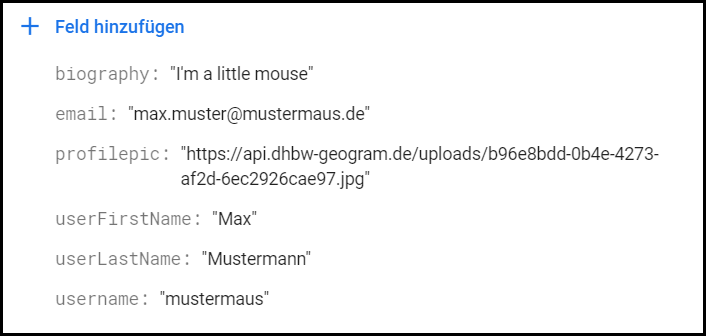
\includegraphics[width=.7\linewidth]{images/collection_users.png}
    \caption{Felder eines \glqq users\grqq{}-Dokumentes}
    \label{fig:users_collection}
\end{figure}

Die Dokumente der Sammlung \glqq images\grqq{} bilden die verschiedenen Bilder von Geogram ab. Ein Bild wird durch folgende Felder definiert:

\begin{itemize}
    \item \textbf{description}: Beschreibung des Bildes
    \item \textbf{id}: Eindeutige Id für das Bild
    \item \textbf{location}: GPS-Informationen für das Bild
    \item \textbf{timestamp}: Zeitpunkt des Hochladens des Bildes
    \item \textbf{title}: Titel des Bildes
    \item \textbf{url}: URL zu dem Bild, welches im Foto-Server abgespeichert ist
    \item \textbf{user}: Username des Bild-Inhabers
\end{itemize}

In \autoref{fig:images_collection} ist ein beispielhaftes images-Dokument abgebildet.

\begin{figure}[H]
    \centering
    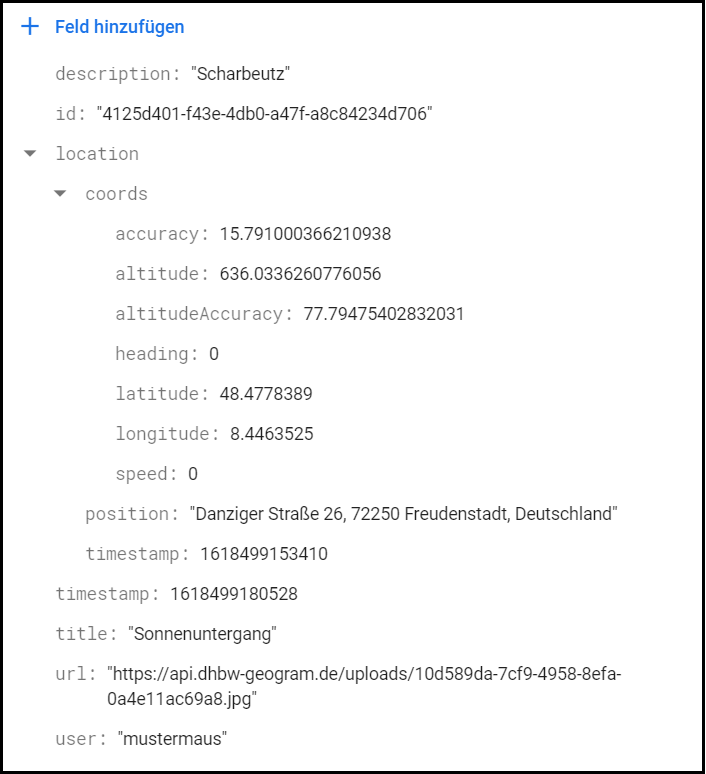
\includegraphics[width=.7\linewidth]{images/collection_images.png}
    \caption{Felder eines \glqq images\grqq{}-Dokumentes}
    \label{fig:images_collection}
\end{figure}